\documentclass{article}
\usepackage[utf8]{inputenc}
\usepackage{hyperref}
\usepackage{listings}
\usepackage[inline]{enumitem}
\usepackage{graphicx}
\usepackage{float}
\usepackage{xcolor}

\hypersetup{
    colorlinks=true,
    linkcolor=black,
    filecolor=magenta,      
    urlcolor=blue,
}


\definecolor{codegreen}{rgb}{0, 0.4, 0}
\definecolor{codegray}{rgb}{0.5,0.5,0.5}

\lstdefinestyle{mystyle}{
    commentstyle=\color{codegreen},
    keywordstyle=\color{blue},
    numberstyle=\tiny\color{codegray},
    stringstyle=\color{orange},
    basicstyle=\ttfamily\small,
    breakatwhitespace=false,         
    breaklines=true,                 
    captionpos=b,                    
    keepspaces=true,                 
    numbers=left,                    
    numbersep=5pt,                  
    showspaces=false,                
    showstringspaces=false,
    showtabs=false,                  
    tabsize=2
}

\lstset{style=mystyle}

\title{Analysis of Brand Prevalence in Digital Video Content using Scale-Invariant Feature Detection}
\date{2020-5-01}
\author{Frederik Gram Kortegaard}

\begin{document}

\maketitle
\pagenumbering{gobble}
\newpage
\tableofcontents
\newpage
\pagenumbering{arabic}

\section{Abstract}
\section{Introduction}
\paragraph{}
Digital content such as videos has quickly risen to become one of the primary marketing platforms
of our day. With this development, advertisements have quickly become an ingrained part of content
itself, this is especially true in the age of Adblockers, now making many traditional digital
ads obsolete. In turn, this has made quantifying the efficacy and value
of advertisements harder to estimate. 
\newline\newline
In the following post, we will be
looking at detecting and validating frame-accurate counts of branding
material in digital media such as videos. Furthermore, we are going to
combine this data, with time stamped user-interactivity data, view counts
and viewerbase demographics.
\newline\newline
If you were to only read a few parts of this paper, I would recommend
reading the section on \textbf{\textit{Detection Models}}, and atleast skimming the visualizations
in \textbf{\textit{Extracting Insight}}. It is important to note that this paper is intended as
a walkthrough of a rapidly developed Proof-of-Concept. Because of this, there will be things 
that could be done more efficiently or elegantly, however, that is not the matter
of the paper.

\section{Data Collection}
\paragraph{}
For this prototype, I have decided that analysis will be done on video content, specifically,
Videos-on-Demand (VODs'), from the popular streaming site \href{http://www.sharelatex.com}{twitch.tv}. 
This is reasoned by the current influx of marketing through streamed media, and the rise of e-sports.
As per the nature of VODs', we will not be analysis content in real-time. However, a brief
explanation of how to do so, will be made later.


\subsection{Fetching Videos}
\paragraph{}
Firstly, it is important to note, that the \textit{rights} to these videos, is not neccesarily
such that downloading them would be considered legal. Thusly, i recommend that this be done only
using your own test-content.
\newline\newline
When fetching videos, there are alot of metric to be considered, some of which being
encoding, filetypes, scaleability and throttling.
All of which become very important, if you were to scale this prototype into a useable
business application. But since we are not doing that, some compromises will be made.


\subsubsection{Youtube-dl}

To download our videos, we are going to use the Python-Bindings for the popular command-line program
\href{https://ytdl-org.github.io/youtube-dl/index.html}{youtube-dl}. There is not alot to say
about this approach, as the python implementation is quite simple, and allows us to very
quickly make a working script, that looks like this:

\begin{lstlisting}[language=Python]
""" Twitch Video-On-Demand Downloader
"""
import os, sys, youtube_dl
from typing import Dict, Tuple

def download_vod(video_id: int, path_to_output_dir: str) -> Tuple[str, Dict]:
  """ Downloads a Twitch VOD referenced by its Twitch ID
      Curtesy of jaimeMF @ https://stackoverflow.com/a/18947879  
  """
  
  ydl_opts = {
      'outtmpl': os.path.join(path_to_output_dir, f'{str(video_id)}.mp4')
      }

  with youtube_dl.YoutubeDL(ydl_opts) as ydl:
      result = ydl.extract_info(
          f"https://www.twitch.tv/videos/{video_id}",
          download = True
      )

  if 'entries' in result:
      # Can be a playlist or a list of videos
      video = result['entries'][0]
  else:
      # Just a video
      video = result
      
  return (os.path.join(path_to_output_dir, f'{str(video_id)}.mp4'), result)

if __name__ == "__main__":

  # Quick CLI Implemenation
  filename = download_vod(
      sys.argv[1], # Video ID
      sys.argv[2]  # Output Dir
  )[0]

  print(f"Finished Downloading VOD to path: {filename}")
\end{lstlisting}
Calling this function, will \textit{not} return, before the video is fully downloaded.

\subsubsection{Conversion to Frames}
Now that we have downloaded our video, we need to convert it to a series of frames. 
For our implementation, we will use the Python bindings for OpenCV2, and use its cv2::VideoCapture object.
this will allow us to iteratively step-and-read through a given video, and yield each frame
as a PIL / OpenCV2 Image object.  This will be useful for the pipeline process later. 
Alternatively, when used as a standalone script, we save the frames to a folder.
\newline\newline
During this process, we are also converting the frames to grayscale, as this
will both reduce the size of our images, and reduce the dimensionality of our data
for our detection model. The code for this simple script, looks like this:
\begin{lstlisting}[language=python]
""" Convert a video to a series of frames using OpenCV
"""
import os, sys, cv2
from typing import Iterable

def to_grayscale_frames(path_to_video: str) -> Iterable:
  """ Convert a video to a series of grayscale frames using OpenCV """
  
  video_capture = cv2.VideoCapture(path_to_video)
  success, image = video_capture.read()
  while success:
    gray = cv2.cvtColor(image, cv2.COLOR_BGR2GRAY)
    yield gray
    success, image = video_capture.read()

if __name__ == "__main__":
  """ Python -m video_to_frames.py
        path_to_video
        output_dir
  """
  # Quick CLI Implemenation
  for enum, frame in enumerate(to_grayscale_frames(sys.argv[1])):
    cv2.imwrite(os.path.join(sys.argv[2], f"{str(enum)}.jpg"))

  print(f"Finished Downloading frames to dir:{sys.argv[2]}")
\end{lstlisting}
Using this function, we can both download every frame to a folder, as a .jpg file. Or we can
stream them, using the method as a generator. This allows us greater flexibility when it comes to easily 
plugging different scripts together in our pipeline, that will be mentioned later.

\section{Detection Models}
\subsection{Requirements}
\paragraph{}
On first thought, it seems quite trivial to detect images 
in videos, when we already know which images we are supposed
to look for. However, this problem is highly domain-specific.
For this project, we are targeting e-sports media, and in this domain,
problems such as images that are embedded
into game maps, partially covered by in-game decals such as
artifacts, noise or more specifically blood or soot, would
be prone to faults using naive image detection.  
\newline\newline
Furthermore, problems might arise by the nature of
scale-invariance or rotation.  
Though this problem is easier to solve using conventional
image detection, it is still a major contributor to instability
of our solution if we were to scale it up to be business
applicable.  So how are we going to solve this problem? 
We know that we need:

\begin{enumerate}
  \item Ability to detect images in other images
  \item Be able to approximate likeness even when images are partially covered. 
  \item Not have scale, skew or rotation significantly degrade our predictive abilities
\end{enumerate}
From here, we are going to look at different detection
techniques, from classical computer vision to the newly
arrived convolutional neural networks, and see if we can
find a solution that fulfills our requirements


\subsection{Possible Solutions}
\paragraph{}
There are several approaches to this problem, but here we will describe a few:
\paragraph{Optical Character Recognition} \mbox{}\\

OCR is a tried and true way of detecting text in images,
however, the ease of use and the high level of accuracy is
not particularly useful to us. Remember, flexibility is one
of our primary concerns.  Barring the issue of non-text based
logos, OCR is also notoriously bad at handling noise. For
these reasons, we are going to dismiss the possibility of
using OCR as our primary tooling for our implementation.

\paragraph{Feature Detection} \mbox{}\\

This is a rather vague title forclassic image detection
algorithms.  The reasoning behind the specificity is a
result of the vast and nauseating sea of Computer Vision
algorithms. If you are interested in hearing more about the
other classical techniques that were not chosen for this
implementation, see the section \textbf{\textit{Other Approaches}}
\newline\newline
Feature Detection typically describes algorithms in which we
use information, such as images, to create new information of
a higher-abstraction.  You could here imagine converting a
16x16 matrix of RGB values, into a two bit binary representing
shapes such as {square, circle, triangle, hook} all of which
are grayscale.  This would allow us to later use this simplified
and “compressed” version of the original data to infer more
complex ideas.  This is, in spirit, the same approach that
Convolutional Neural Networks use, however with classical
techniques we are typically more actively participating in
deciding these abstractions instead of having the neural
networks black box make its own decisions.  Conversely we are
also limited by our own ability to extract meaningful patterns
and by reason of man-power and a less pure-mathematical
approach, it is also harder to validate the efficiency of
large-scale data.

\paragraph{Neural Networks} \mbox{}\\

Neural networks such as CNNs’ and RNNs’  have a few benefits,
such as allowing us to train models with a modicum of
generalization built-in. However, there are also a wealth of
issues such as:

\begin{enumerate}
  \item Trusting the black box
  \item Training Multiple Models
  \item Collecting \textit{a lot} of data, for every logo.
\end{enumerate}

A more in-depth explanation of the models can be found in
the section: \textbf{\textit{Neural Networks, a deeper look.}}  So, are these
problems insurmountable? Are they worth the pain to become
an “AI Solution”?

\subsection{Picking a Model}
\paragraph{}
Based on the former descriptions, and experience working
with these different techniques, I came to the conclusion that
Neural Networks. at least not for the scale that we are thinking
in for thsi implementation, is not worth it. There are plenty
of great parts about the approach, one of
which is multi-objective learning, and multiclass
classification. Approaches that allow us to train a
singular neural network, to perform different but similar
tasks (such as looking for a variety of logos in a single
image) and exploit the commonalities in the tasks to improve
accuracy across the board. This sounds amazing! Right? Well,
yes, however, if we sideline the lacking technology and our
limited project scope, this would still require us to either
create a supervised-training set for each of our logos, to
train our model with. Or, we would need a way to validate
our classification post-prediction.  Both of these tasks
take a lot of manpower, and are not very scalable solutions.
As reasoned by this, we come to the conclusion that for this 
project, sticking with a more classical approach is better
aligned with our scope and resources.

\section{Scale-Invariant Feature Detection}
\paragraph{}
The feature detection algorithm we are going to use for this project is called SIFT (Scale-Invariant Feature Detection).  Before continuing on, it is important to note here, that this algorithm is patented by David Lowe, and requires a license to use commercially.   
\subsection{How It Works}
\paragraph{}
Our SIFT algorithm is firstly given an image, in our case,
an image of the logo we want to detect. From this image,
SIFT collects a group of keypoints, also described as points
of interest. These points usually represent areas with very
unique attributes such as lines of various angles, textures
and clear-separations (such as a mountain peak seperating
from the background).
\newline\newline
Mathematically this works by convolving
the image using gaussian filters at different sizes, the areas
of which have the minima / maxima difference between these
different convolutions are said to be the most unique, and
are stored in a database for future use.
\newline\newline
This technique has to be done for every logo we want to detect, however, in comparison to the neural solution we mentioned earlier, this is completely unsupervised.  
After having found this set of keypoints, we now have to “thin out the bunch” a bit, since the aforementioned technique, known as “Scale-space extrema detection” creates a lot of keypoints, some of which of questionable robustness.  This process, called keypoint localization is done via. the following list of techniques:

\begin{enumerate}
  \item Interpolation
  \item Contrast Filtering
  \item Edge Sensitivity
\end{enumerate}

As the first step, we are going to interpolate nearby keypoints using the quadratic Taylor expansion. This is done for every keypoint that we found previously, in an attempt to more precisely calculate their position. This process helps counteract the unstable nature of our massive collection of keypoints.  
\newline\newline
Following this, we are going to discard every keypoint whose second order Taylor expansion is lower than 0.03, which results in a dramatic decrease in keypoints in areas such as the sky, as the contrast of keypoints relative to the surrounding area could correlate with its descriptiveness and uniqueness in the image.  Lastly, we are tackling a problem relating to our Difference-of-Gaussian function (The same function used in Scale-space extrema detection). This procedure responds very strongly to edges, no matter the stability of its position. To solve this, we are filtering out keypoints whose locations have been poorly determined, but still created a high edge response.    
\newline\newline
Now that we have done some filtering on our keypoints, it is time to make our features rotation-invariant. This is done by assigning each keypoint with at least one orientation, based on the gradient directions of its locale in the image. The calculations done in this process, takes the keypoints scale into consideration, which in return, creates the scale-invariant nature of the algorithm.  For the final step of the algorithm, we compute descriptor vectors for each of our keypoints, which creates even more invariance to factors such as lighting and view angle.
\newline\newline
As our understanding of our approach is now solid enough to build a prototype of our project, let us move on to the implementation of the SIFT algorithm in the programming language Python.
\subsection{Implementation Details}
kdtrees, flann etc etc
\subsection{Code}
\lstinputlisting[language=Python]{../src/brand_prevalence/processing/sift.py}


\section{Extracting Insight}
\subsection{Viewer Interaction}
\paragraph{}
Knowing how many frames of exposure your brand is
getting for any given content, can be very valuable
information when analysing the efficacy of marketing. However,
imagine that every single one, of those frames, were during a "bathroom break"
or something of the likes. In this situation, we could reasonably assume, that
there will be given less attention to the video, and thus, the frames of exposure you are getting,
that otherwise.
\newline\newline
To try and partially mitigate this, we are going to look at the
user interactivity data, for any given timeframe of the video. Though it might be an assumption,
i find it fair, that more posts would be made in the chat of a video, in times where something attentiongrabbing has just, or is about to occur.
And thus, these timeframes can give us approximate "areas of higher attention".


\subsubsection{Fetching Chat Data}
\paragraph{}
Following the rapid-prototyping methodology
that we have stuck to, during this project, we are again going
to use a pre-made solution by Petter Kraabol which he creatively
dubbed: \href{https://github.com/PetterKraabol/Twitch-Chat-Downloader}{“Twitch-Chat-Downloader”}.  
\newline\newline
This command-line tool allows us to download the complete
chat-history related to a video, using
either preset or custom formats.  We are largely only interested
in the exact time each comment was posted, and not the duration of
which it stayed in the chat, and thus we are going to use the built-in
format “irc”, which might be familiar to a few of you. 
\newline\newline
Visually, it looks like this:  [timestamp] <username> comment. 
This format is rather simple, but it gives us all the information
we need. And as for the implementation, we used Python's subprocess
library to use interact with the tools CLI, and converted that to a python function like this:

\begin{lstlisting}[language=python]
""" Simple interface to use
  PetterKraabol's Twitch-Chat-Downloader
  # https://github.com/PetterKraabol/Twitch-Chat-Downloader
"""
import os, sys, subprocess

def download_twitch_chat(video_id: int, path_to_output_dir: str, twitch_id: str) -> str:
  """ Downloads the given Twitch VODs
      chat as irc format """
  # Start subprocess
  p = subprocess.Popen([
      "tcd", "--video", str(video_id),
      "--format", "irc",
      "--output", path_to_output_dir,
      "--client-id", twitch_id],
      shell=True)
  # Wait for subprocess to finish
  p_status = p.wait()

  return os.path.join(path_to_output_dir, f"{str(video_id)}.log")

if __name__ == "__main__":
  # Quick CLI Implemenation
  filename = download_twitch_chat(
      sys.argv[1], # Video ID
      sys.argv[2], # Output Dir
      sys.argv[3]  # Twitch ID
  )
  print(f"Finished Downloading Chat log of VOD {sys.argv[1]} to path: {filename}")
\end{lstlisting}
Here it is important to note the argument \textit{Twitch ID}, this is
the Twitch Developer ID, and can be found at \href{https://dev.twitch.tv}{dev.twitch.tv}. Without this, we will not be
able to download the full chat log, only part of it.
\newline\newline
A snippet of the downloaded chat log can be seen here:
\lstinputlisting[language=Python, firstline=0,lastline=10]{../src/brand_prevalence/output/589455713.log}

\subsubsection{Ensuring Uniqueness}
\paragraph{}
We cannot naively trust that the volume of
comments is a good indicator of neither the intensity
of which the users are watching the stream, nor the amount
of unique impressions one can except by having exposure
during that given timeframe.  Given this problem, we can
start filtering out “spam” comments, by setting a minimum
time between posts, before we decide to include them in our
calculations.  For this project, we decided that a heuristic
of ten seconds gave us good results.
\newline\newline
With this consideration, we can quickly visualize
the size disparity of our dataset, given different
heuristic values:
\begin{figure}[H]
  \centering
  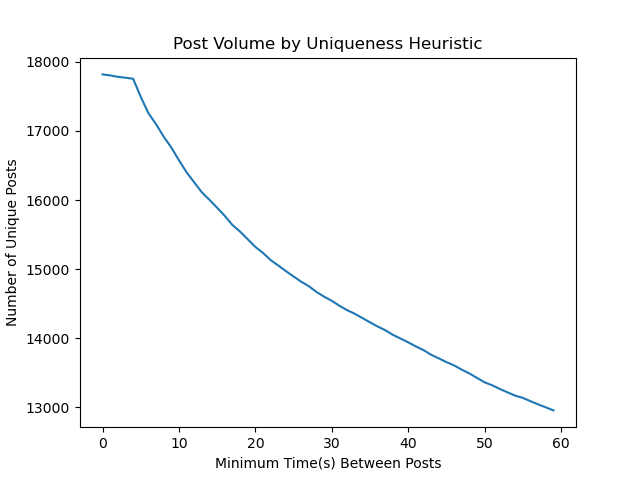
\includegraphics[width=\linewidth]{./resources/chat_activity_uniqueness.png}
\end{figure}
As you would expect, setting our heuristic to zero sharply increases our volume of unique posts. And as for our example, spam only decreased our dataset by cirka. 2000 posts, around an 11 percent decrease from our total volume of posts. 
\newline\newline
Based on this, we can conclude that the measure of uniqueness can definitely contribute to creating robust and trustable data, however, it is not necessary to gain value, as long as there is still awareness regarding spam, when looking at numbers.
The function used to collect this data, will also be mentioned in later functions, and looks like this:
\begin{lstlisting}[language=python]
  def _make_unique(path_to_chat_log: str, UNIQUENESS: int = 10) -> Dict:
    """ Converts a given chat log to
        a spam-filtered dictionary, 
    """

    USER_POST_TRACKER = defaultdict(int)
    posts = defaultdict(int)

    for enum, post in enumerate(open(path_to_chat_log, 'r', encoding="utf8").read().split('\n')):
        post = post.split(' ')
        if not len(post) >= 2:
            continue

        timestamp, username = post[0], post[1]
        timestamp = _to_seconds(timestamp)

        # if the post was created withing UNIQUENESS seconds
        # since the last counted post by the same user,
        # ignore it.
        if abs(timestamp - USER_POST_TRACKER[username]) 
          <= UNIQUENESS:

            print(f'''
              Ignoring comment number: {enum} 
              from user "{username}"'''
            )
            continue
        # Otherwise, count it and update the timestamp.
        else:
            USER_POST_TRACKER[username] = timestamp
            posts[str(timestamp)] += 1

    return posts
\end{lstlisting}
In this code, we use the function \textit{\_to\_seconds()}, which simply converts
the string timestamps as mentioned in the previous section, to an integer, representing it purely
by seconds into the video.
\subsubsection{Visual Analysis}
The simplest approach to gain insight from this data,
would be to simply overlay chat-activity data on-top of
a timeline of when our brand is visible (detected by our
SIFT Algorithm). To do this, we are going to use the Python
library \href{https://matplotlib.org/}{matplotlib}.
\newline\newline
Firstly, we are going to plot the volume of posts
created (Y axis), by the number of seconds into the
stream they were posted (X axis). For this, we are using
the function matplotlib::pyplot.plot, and feeding it our
data, as well as using the marker style “.r”, which ensures
that each individual point on the X axis, will be marked by
a red circle, and the points will be connected by a red line.
\begin{figure}[H]
  \centering
  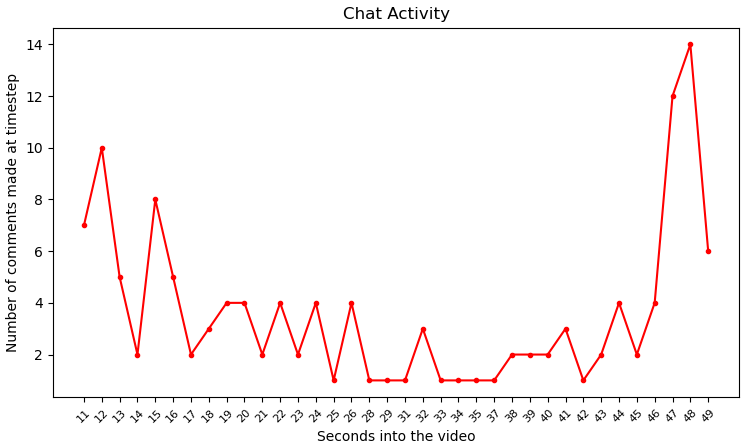
\includegraphics[width=\linewidth]{./resources/chat_activity_pr_second.PNG}
\end{figure}

Hereafter, we want to overlay the time frames in which
our brand logo is visible. This is achieved by simply
going through each entry in our bounding\_boxes.json file,
dividing each frame number by 60 (Our video is 60 frames
per second, thusly this will give us the number of seconds
into the video the entry represents), and then plotting the
entries in a similar fashion as our post volumes.
Matplotlib will by itself handle connecting points
next to each other, with a blue line. 

\begin{figure}[H]
  \centering
  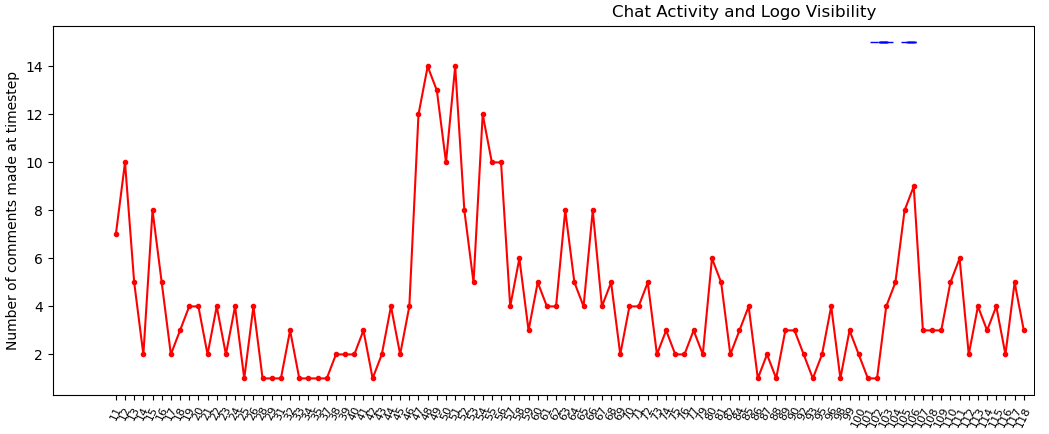
\includegraphics[width=\linewidth]{./resources/chat_and_logo_visibility.png}
\end{figure}

Finally, now that we have our illustrations, we
can try to draw some conclusions based on our dataset.
We see that our logo was visible from 102 to 104, and
again from 105 to 106, given that this is a visual analysis,
we have not yet accounted for the accuracy of our detection
model, and thus, we can safely assume that this is one
connected timeframe of exposure, from 102 to 106.
\newline\newline
Given this, we can see that our logo gained exposure during a timeframe of medium to medium-high chat activity, which can correlate with the “clip-ability”, or rather, how many times that specific timeframe will be rewatched or reposted and furthermore, we can assume that chat interactivity correlates with the intensity or focus the viewerbase is giving the stream. 

Converting our data into visual representations is vital for our application,
luckily for us, it is also quite simple, as seen in the code we used to generate the graphs shows earlier:

\begin{lstlisting}
def timeframe_chat_activity(path_to_chat_log: str, path_to_bounding_boxes: str):
  """ Creates a matplotlib plot showing the chat activity
      and the timeframes of branding exposure together.
  """

  posts = _make_unique(path_to_chat_log, 10)
  fig, ax = plt.subplots()

  ax.plot(list(posts.keys()), list(posts.values()) , '.r-')

  # Plot timeframes in which bounding boxes are visible
  for key in list(json.load(open(path_to_bounding_boxes, 'r')).keys()):
      ax.plot(int(key) / 60, max(list(posts.values())) + 1 , '_b-',)

  plt.title("Chat Activity and Logo Visibility")
  plt.xlabel("Seconds into the video")
  plt.xticks(fontsize=8, rotation=65)
  plt.ylabel("Number of comments made at timestep")

  return plt
\end{lstlisting}

\subsubsection{Numerical Analysis}
\paragraph{}
Now that we have both generated and looked over our visual data, its time for hard numbers. Questions that might have risen from our previous chapter, such as:
\textit{"How big a percentage is that?} or
\textit{"How big was the total?}.
Well, lets calculate it. First and foremost, we are interested in how big of a percentage of the chat-activity existed withing the bounds of
our branding being visible. As we have data telling us the times of both exposure and posts, we simply count it up,
using the following function:

\begin{lstlisting}[language=python]
def percent_of_chat_activiy(path_to_chat_log: str, timeframes: List[Tuple[int]]) -> float:
  """ Returns the total percentage of chat activity
      experienced during the given timeframes
  """ 

  # Filter by Uniqueness
  posts = _make_unique(path_to_chat_log, 10)
  total_posts = sum(posts.values())
  timeframe_posts = list()
  
  # Iterate through timeframes
  for enum, timeframe in enumerate(timeframes):
      posts_during_timeframe = sum(
        [posts[str(timestamp)]
        for timestamp in timeframe]
      )
  
      percent = posts_during_timeframe / total_posts * 100
      timeframe_posts.append(posts_during_timeframe)

  return sum(timeframe_posts) / total_posts * 100 
\end{lstlisting}
Following this, and with the addition of some nice output formatting, 
you end up with returns like this:

\begin{verbatim}
  >> There are a total of 5432 comments in the given chat log
  >> timeframe: 0, saw a total of 432 posts, which is 7.952% of the total chat activity
  >> timeframe: 1, saw a total of 241 posts, which is 4.436% of the total chat activity
  >> ...
  >> Collectively, the 26 timeframes got 46.342% of the chat activity
\end{verbatim}

Given theese results, we can start to gather a better picture of how 
much \textit{actual} exposure (using our assumption of attention)
our branding received. Let os combine this with another numerical data point,
the percentage of the total video, our received exposure makes up.
This data can be used to fuel our intuition, and when combined with the
previous data point, be used for further calculations at higher levels of abstraction.
We will in a later section dive into higher-abstraction analysis, but for now, let us look at the
function used to calculate this data:

\begin{lstlisting}[language=python]
def exposure_as_percent_of_video(path_to_bounding_boxes: str, video_lenght_in_seconds: int, fps: int = 60) -> float:
  """ Returns what percentage of a videos lenght
      the given logo was visible in.
  """
  
  # Load bounding boxes
  boxes = json.load(open(path_to_bounding_boxes, 'r', encoding='utf8'))

  # Calculate Percentage
  percent = ((1 / fps) * len(boxes.keys())) / video_lenght_in_seconds * 100

  return percent
\end{lstlisting}

This simple function, with some pretty-printing as before, will return data
in the following manner:
\begin{verbatim}
  >> the timeframes in bounding_boxes.json make up 23.422% of the total video
\end{verbatim}

Now, these numbers might not seem very exciting, knowing the percentage of chat activity, really does not allow
us to conclude much. The percentage of total video lenght is neat, but again, tells us very little
about the \textit{clip-ability} or \textit{high-attention} probability of the timeframes
in which our brand got exposure, however, when combined, we get a clearer picture.
\newline\newline
Knowing that our video was exposed for e.g. 13\% of the total video, but received
more than 60\% of the chat activity, is robust enough to start forming some
ideas about \textit{what} content our brand actually got exposure in. And yes,
we can pretty confidently assume, that this was not during a bathroom break.


\subsection{Selective Viewcounts}
Now that we got through a more, assumptious, segment of our analysis. Let us
look at some data, that is unequivocally useful, and really should be a part
of the standard analytics-platform these video sites have.
\newline\newline
Given a video, without analysing the video in real-time, it is hard to know
how many views our timeframes of exposure actually got, sure, we can approximate
using the chat activity and the total view count, but that is not good enough. We need
to know how many views each individual frame received.
\subsubsection{Example}

\section{Scaleability}
\subsection{Piping}
\subsubsection{Code}

\subsection{Microservices}
\subsubsection{Implementation}

\subsection{Load Balancing}
\subsubsection{Implementation}

\section{Insight Useability}
\subsection{Generating Reports}
\subsection{Example}
\subsection{Code}

\section{Conclusion}

\end{document}